\section{Optimalizácia prevádzky dynamických systémov}
Optimalizácia je prostriedok, ktorým sa dosiahne najlepší výsledok za daných okolností. Pri navrhovaní, stavbe a údržbe akéhokoľvek inžinierskeho systému, musia inžinieri prijať mnoho technologických a manažérskych rozhodnutí v niekoľkých fázach. Konečným cieľom všetkých takýchto rozhodnutí je buď minimalizovať potrebné úsilie alebo maximalizovať požadovaný úžitok. Pretože úsilie alebo úžitok, požadovaný v akejkoľvek praktickej situácii, môže byť vyjadrený ako funkcia určitých rozhodovacích premenných, optimalizácia môže byť definovaná ako proces hľadania podmienok, ktoré poskytujú maximálnu alebo minimálnu hodnotu funkcie. Na Obr. \ref{fig:cost_fun_ex} môžeme vidieť, že ak bod $ x^{\star} $ zodpovedá minimálnej hodnote funkcie $ f(x) $, rovnaký bod zodpovedá maximálnej hodnote negatívnej hodnote $ -f(x) $ tej istej funkcie. V tom prípade môžeme optimalizáciu bez straty zovšeobecniť na proces minimalizácie, pretože maximum funkcie dokážeme nájsť ako minimum negatívnej hodnoty rovnakej funkcie \cite{rao:intro_engin_opt:2009}. 

\begin{figure}
	\centering
	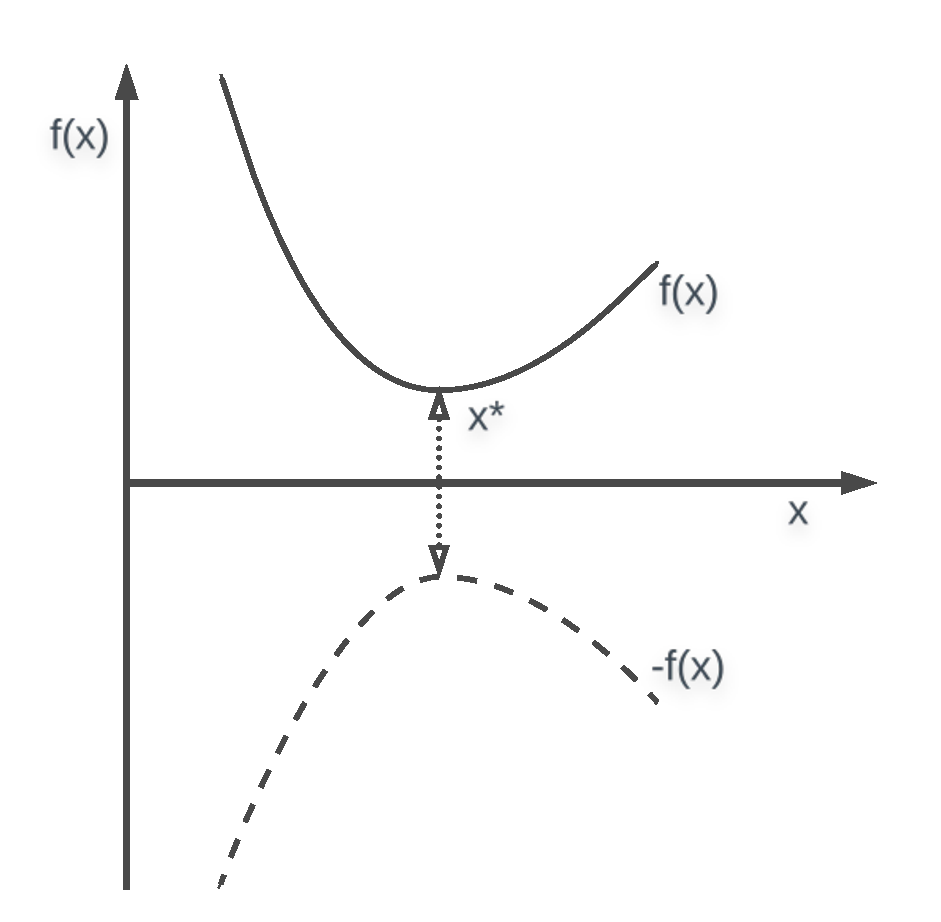
\includegraphics[width=0.5\linewidth]{images/optimization_obj}
	\caption{Minimum účelovej funkcie $ f(x) $ je v rovnakom bode ako maximum $ -f(x) $.}
	\label{fig:cost_fun_ex}
\end{figure}

Pri návrhu optimalizačného problému, môže nastať niekoľko situácii -- (a) v najlepšom prípade získame neohraničenú optimalizačnú úlohu, (b) budeme mať ohraničenia v tvare rovnosti alebo (c) zakomponujeme aj ohraničenia v tvare nerovností. Všetky tieto problémy sa často vyskytujú pri riešení efektivity zariadenia a nazývajú sa problémy statickej alebo
% RP: parametricka optimizalizacia je nieco trochu ine
parametrickej optimalizácie \cite{agrawal:static_opt:1999}. Statická je preto, lebo
% RP: x by zom skor volal premenne. moze sa to byt 
parametre $ x $ účelovej funkcie $ f(x) $ sú nezávislé od času, nemenia sa. 

Majme všeobecný dynamický systém, ktorý vieme opísať nasledovným modelom
\begin{equation*}
	\der{x}{t} = f(t, x, u, \theta),
\end{equation*}
kde $ x $ sú stavy systému, $ u $ je riadiaca veličina a $ \theta $ predstavuje parametre modelu. Potom ak definujeme účelovú funkciu $ \ell_e(\bar{x},\bar{u}) $, ktorá vyjadruje ekonomickú kvalitu systému, môžeme získať optimálne ustálené stavy $ \bar{x}^{\star}, \bar{u}^{\star} $ ako
\begin{equation}
	\begin{split}
		\min_{\bar{x},\bar{u}}& \quad \ell_e(\bar{x},\bar{u}), \\
		% RP: Ak maju byt optimalizovane ustalene stavy, tak \dot x = 0
		% RP: Ak su optimalizovane premenne \bar x a \bar u, tak by sa mali vyskytovat vo vsetkych obmedzeniach 
		\text{s.t.}& \quad \dot{x} = f(t, x, u, \theta) \\
		& \quad x_{\min} \leq x \leq x_{\max} \\
		% RP: tu ma byt asi u, nie x
		& \quad u_{\min} \leq x \leq u_{\max}
	\end{split}
	\label{eq:econ_opt_dyn_sys}
\end{equation}
ktoré zaručia, že daná účelová funkcia bude dosahovať minimum v danom bode \cite{hernandez:economics_opt_w_mismatch:2019}. Takýmto spôsobom dokážeme na základe statickej optimalizácie optimalizovať prevádzku akéhokoľvek dynamického systému. Treba však zdôrazniť, že celá táto problematika je založená na poznaní matematického opisu zariadenia. V prípade, že model nebude ekvivalentný so skutočným zariadením (čo v podstate nikdy nie je), získané výsledky nebudú optimálne, v horšom prípade môžu narušiť celé fungovanie zariadenia. To ako sa vysporiadať s touto problematikou vysvetlíme v nasledujúcich častiach.

\subsection{Dvojkroková optimalizácia}
% RP: "Je to metóda" toto nie je vhodny styl na zaciatok odstavca, toboz podkapitoly
Je to metóda, ktorá pozostáva z
% RP: Myslim, ze cislovky by sa mali pisat slovom
2 krokov, resp. z 2 optimalizačných úloh. V prvom kroku, na základe nameraných údajov vstupov $ u $ a stavov $ x $ resp. výstupov $ y $, odhadneme neznáme parametre modelu, ktorý opisuje náš dynamický systém. Túto optimalizačnú úlohu by sme mohli sformulovať podobne ako uvádza rovnica \ref{eq:param_est_opt_form}. V druhom kroku využijeme informácie z tohto modelu, napr. informácie o ustálených stavoch $ \bar{x} $, na výpočet optimálnych ustálených hodnôt $ \bar{x}^{\star}, \bar{u}^{\star} $, ktoré môžeme aplikovať na naše zariadenie. Takúto problematiku by sme mohli sformulovať ako v prípade \ref{eq:econ_opt_dyn_sys}. V princípe je možné tento cyklus zopakovať niekoľkokrát, pričom po každom cykle by sme mali získať presnejšie výsledky vzhľadom na daný model.

% RP: skor "v rozdiele" ako "v rozdiely"
V skutočnosti táto metóda nerieši problém v rozdiely medzi skutočným zariadením a modelom, i keď v určitých prípadoch dokážeme ladením parametrov modelu zmenšiť tento rozdiel.

\subsection{Schéma úpravy modifikátora}
V prvom rade treba uviesť, že ide o metódu, ktorá jednak hľadá optimum prevádzky dynamických systémov a jednak rieši problematiku rozdielu nominálneho modelu od skutočnosti. Okrem iného ide o techniku, ktorá má uplatnenie v dynamickej optimalizácii a
% RP: "v posledných rokov"
v posledných rokov nadobudla na významnosti \cite{marchetti:modifier_adapt_scheme:2020}.

Schéma úpravy modifikátora (\textit{angl. \aps{Modifier Adaptation Scheme}}) je iteračná metóda, ktorá ma skvelé uplatnenie v reálnom živote. Hlavnými črtami sú spôsob, akým sa merania používajú na korekciu nominálneho modelu, a úloha, ktorú neskôr model zohráva pri výpočte ďalších vstupov.

Princíp tejto metódy spočíva v úprave gradientu účelovej funkcie nominálneho modelu $ \nabla_N\ell_e(\bar{x},\bar{u}) $ následovným štýlom
\begin{equation}
	\nabla J = \nabla_N\ell_e(\bar{x},\bar{u}) + \lambda_k,
\end{equation}
kde $ \lambda_k $ predstavuje hodnotu modifikátora v $ k $-tom kroku. Upravený gradient po integrácii má tvar 
\begin{equation}
	J^{\tiny{(MA)}} = \ell_e(\bar{x},\bar{u}) + \lambda_ku.
\end{equation}
Hodnota modifikátora v $ k $-tom kroku je určená na základe váhovania dvoch faktorov. Určitú časť prispievajú minulé hodnoty modifikátora $ \lambda_{k-1} $ a zvyšnú časť tvorí rozdiel v gradientoch účelových funkcii $ \Delta_{k-1} $ skutočného zariadenia a nominálneho modelu 
\begin{equation}
	\label{eq:mas_weight}
	\lambda_k = c\lambda_{k-1} + \left(1 - c\right)\Delta_{k},
\end{equation}
kde $ c $ je váhový koeficient, ktorý môže nadobúdať hodnoty $ c \in \lbrace 0; 1 \rbrace $ v závislosti od toho, či chceme aby sa modifikátor menil viac alebo menej s pribúdajúcimi dátami.
% RP: skor "hodnotu premennej" ako "Samotnú premennú"
Samotnú premennú $ \Delta_k $ je náročné určiť správne, pretože obsahuje gradient účelovej funkcie reálneho zariadenia $ \nabla_P\ell_e(\bar{x},\bar{u}) $, ktorý
% RP: "mi nemáme"
mi nemáme k dispozícii a preto je nutné ho odhadnúť napr. v takejto podobe
% RP: Kludne by som tu jasne povedal, ze sa jedna o metodu konecnych rozdielov.
\begin{equation}
	\nabla_P\ell_{e,k}(\bar{x},\bar{u}) = \frac{\ell_{e,k}(\bar{x},\bar{u}) - \ell_{e,k-1}(\bar{x},\bar{u})}{\bar{u}_k - \bar{u}_{k-1}}.
\end{equation} 
Potom $ \Delta_k $ môžeme definovať ako 
\begin{equation}
	\label{eq:mas_correction}
	\Delta_k = \nabla_P\ell_{e,k}(\bar{x},\bar{u}) - \nabla_N\ell_{e,k}(\bar{x},\bar{u}).
\end{equation}
Treba spomenúť fakt, že práve odhad gradientu účelovej funkcie skutočného zariadenia $ \nabla_P\ell_{e,k}(\bar{x},\bar{u}) $ spôsobuje najväčšie nepresnosti, najmä kvôli šumu merania. 

\subsection{Použitie hybridných modelov}
Hybridné modelovanie si takisto dokáže poradiť s optimalizáciou prevádzky, pričom jasnou výhodou je, že nepotrebuje odhadovať gradient účelovej funkcie, ktorý prispieva najväčšou neistotou metóde úpravy modifikátora. V niektorých vedeckých publikáciach sa ukázalo, že využitie hybridných modelov, pri optimalizácii prevádzky dynamických systémov, výrazne dopomohlo k zvýšeniu efektivity, najmä kvôli lepším predikčným vlastnostiam hybridných modelov \cite{bhutani:hybrid_modelling_opt:2006}. 

Pri zostavovaní optimalizačnej úlohy môžeme vychádzať z rovnice \ref{eq:econ_opt_dyn_sys}, ktorú musíme upraviť tak, aby zohľadňovala danú štruktúru hybridného modelu (Obr. \ref{fig:hybrid_model_general}). V prípade sériového zapojenia by táto optimalizačná úloha mohla vyzerať nasledovne
\begin{equation}
	\begin{split}
		\min_{x,u} &\quad \ell_e\left(x,u\right).\\
		% RP: \dot x = 0
		\text{s.t.} &\quad \dot{x} = f\left(t,x,u,\theta\right)\\
		&\quad \theta = g(u)
	\end{split}
\end{equation}
Dátový model $ g(u) $, ktorý bol vopred natrénovaný na dátach zo zariadenia, odhaduje parametre systému $ \theta $ na základe meniacej sa vstupnej veličiny $ u $. Odhadnuté parametre dopĺňajú
% RP: Skor by som povedal "nominalna" ako "neidentifikovaný"
neidentifikovaný mechanický model $ f(t,x,u,\theta) $, ktorý poskytuje údaje o stavoch $ x $ v účelovej funkcii $ \ell_e\left(x,u\right) $. 

Paralelné zapojenie je trošku odlišné. Jednak vychádza z predpokladu, že nominálny model, ktorý máme je už identifikovaný. Tým pádom dokážeme získať údaje o rozdieloch $ \Delta $ medzi výstupmi zo skutočného zariadenia a nominálneho modelu. Ná týchto dátach je natrénovaný dátový model $ h^{(1)}(u) $, ktorý na základe vstupných údajov $ u $ upravuje výstupy $ x $ z mechanického modelu $ f(t,x,u) $. Optimalizačnú úlohu by sme mohli sformulovať ako
\begin{equation}
	\begin{split}
		\min_{x,u} &\quad \ell_e\left(\hat{x},u\right),\\
		\text{s.t.} &\quad \dot{x} = f\left(t,x,u\right)\\
		&\quad \hat{x} = x + \Delta\\
		&\quad \Delta = h^{(1)}(u)
	\end{split}
\end{equation}
kde $ \hat{x} $ predstavuje upravené výstupy z hybridného modelu.

Sériovo--paralelná štruktúra je akousi kombináciou oboch predchádzajúcich architektúr a optimálne ustálené hodnoty $ \bar{x}^{\star}, \bar{u}^{\star} $ môžeme získať vyriešením  optimalizačnej úlohy v tvare
\begin{equation}
	\begin{split}
		\min_{x,u} &\quad \ell_e\left(\hat{x},u\right).\\
		\text{s.t.} &\quad \dot{x} = f\left(t,x,u,\theta\right)\\
		&\quad \theta = g(u) \\
		&\quad \hat{x} = x + \Delta\\
		&\quad \Delta = h^{(2)}(u)
	\end{split}
\end{equation}
Treba však zdôrazniť, že dátový model paralelného zapojenia $ h^{(1)} $ nie je totožný s dátovým modelom $ h^{(2)} $ kombinovaného zapojenia, pretože v tomto usporiadaní sú dáta o rozdieloch $ \Delta $ odlišné. Je to spôsobené najmä kvôli meniacim sa parametrom $ \theta $ mechanického modelu, ktoré sú odhadované druhým dátovým modelom $ g(u) $. Na druhej strane, dátový model $ g(u) $ môže byť rovnaký ako v sériovom zapojení a často aj býva rovnaký. 
